% Paper introduction: RMA (Kumar et al., RSS 2021).
% Compile from slide/:
%   lualatex -interaction=nonstopmode -output-directory=out rma_legged_robot_en.tex
\documentclass[aspectratio=169,10pt,t]{beamer}
\usepackage[en]{labslide}

\graphicspath{{../paper_tex/rma_legged_robot/figures/}}

\kicker{Paper introduction}
\title[RMA: Rapid Motor Adaptation]{RMA: Rapid Motor Adaptation for Legged Robots}
\subtitle{Adjust the gait to unseen ground and loads in under a second}
\author{Ashish Kumar, Zipeng Fu, Deepak Pathak, Jitendra Malik}
\venue{RSS 2021 \quad UC Berkeley / Carnegie Mellon University}
\date{September 2026}

\begin{document}

\begin{frame}[plain]
  \labtitlepage{%
    \agendacard[blue]{Adapt in real time}{Change the gait before a fall.}%
    \hfill
    \agendacard[orange]{Split policy and estimation}{Finish learning in simulation.}%
    \hfill
    \agendacard[green]{Walk unseen terrain}{No extra real-world training.}%
  }
\end{frame}

\begin{frame}{Problem | Adapt while walking}
  {\footnotesize\color{muted} What changes under the robot: sand, mud, grass, steps, slip, load}

  \vspace{1.15em}
  \begin{columns}[T,onlytextwidth]
    \begin{column}{0.48\textwidth}
      \infocard[orange]{RMA}{Under one second. The gait changes while the robot walks. Learning finishes in simulation, with no extra trials on the robot.}
    \end{column}
    \hfill
    \begin{column}{0.48\textwidth}
      \infocard[blue]{Peng et al.\ (2020)}{Four to eight minutes on the robot. Collecting data before the robot can walk means falls, and falls damage the hardware.}
    \end{column}
  \end{columns}

  \takeaway{Train the gait and the adaptation in simulation, then deploy both unchanged.}
  \source{Kumar et al., RSS 2021, Sec.~1}
\end{frame}

\begin{frame}{Background | The sim-to-real gap is several gaps at once}
  \begin{columns}[T,onlytextwidth]
    \begin{column}{0.32\textwidth}
      \infocard[blue]{Robot and model}{The physical robot and its simulator model differ.}
    \end{column}
    \hfill
    \begin{column}{0.32\textwidth}
      \infocard[orange]{Terrain variety}{Real ground is wider than the terrain used in training.}
    \end{column}
    \hfill
    \begin{column}{0.32\textwidth}
      \infocard[green]{Contact}{Sinking and deformable ground are weak points of a rigid-body simulator.}
    \end{column}
  \end{columns}

  \vspace{1.1em}
  \centering
  {\footnotesize\color{muted} Where the data for estimation is collected}\\[0.55em]
  \begin{tikzpicture}[node distance=5mm]
    \node[kwblue, text width=26mm] (a) {Walk\\4--8\,min};
    \node[kwblue, text width=26mm, right=of a] (b) {Estimate\\parameters};
    \draw[kwarr] (a) -- (b);
    \node[kworange, text width=28mm, right=11mm of b] (c) {History from\\simulation};
    \node[kworange, text width=22mm, right=of c] (d) {Train\\$\phi$};
    \draw[kwarr] (c) -- (d);
    \node[font=\scriptsize, text=muted, above=1.4mm of a] {Earlier adaptation};
    \node[font=\scriptsize, text=muted, above=1.4mm of c] {RMA};
  \end{tikzpicture}

  \takeaway{Keep the data for adaptation inside simulation, and train the estimator there too.}
  \source{Kumar et al., Sec.~1 \quad Peng et al., RSS 2020}
\end{frame}

\begin{frame}{Related work | Robustness, identification, extra real-world trials}
  \begin{columns}[T,onlytextwidth]
    \begin{column}{0.32\textwidth}
      \infocard[blue]{Model-based control}{Accurate dynamics and hand-tuned gaits. MPC on Cheetah 3, inverted-pendulum planning on ANYmal.}
    \end{column}
    \hfill
    \begin{column}{0.32\textwidth}
      \infocard[orange]{Randomized context}{Randomize friction and mass for robustness. Inside that range the gait tends to become conservative.}
    \end{column}
    \hfill
    \begin{column}{0.32\textwidth}
      \infocard[green]{Real-world identification}{Optimize a latent from real rollouts. A fast initialization still leaves several trials at deployment.}
    \end{column}
  \end{columns}

  \takeaway{RMA learns the gait from privileged information, and replaces that information at runtime with recent history.}
  \source{Kumar et al., Sec.~2. Lee et al.\ (2020) are robust on hardware, with a hand-designed trajectory generator and motor model.}
\end{frame}

\begin{frame}{Method | Show the environment only during training}
  \centering
  \begin{tikzpicture}[node distance=3.2mm]
    \node[kwgreen, text width=20mm] (e) {Context\\$e_t$};
    \node[kwgreen, text width=20mm, right=of e] (mu) {Encoder\\$\mu$};
    \node[kwgreen, text width=20mm, right=of mu] (z) {Extrinsics\\$z_t$};
    \node[kwgreen, text width=20mm, right=of z] (pi) {Policy\\$\pi$};
    \node[kwgreen, text width=20mm, right=of pi] (a) {Joint targets\\$a_t$};
    \draw[kwarr] (e) -- (mu);
    \draw[kwarr] (mu) -- (z);
    \draw[kwarr] (z) -- (pi);
    \draw[kwarr] (pi) -- (a);
    \node[font=\scriptsize, text=muted, anchor=south west]
      at ([yshift=1.6mm]e.north west)
      {Phase 1: reinforcement learning. $e_t$ is known only inside the simulator};

    \node[kworange, text width=20mm, below=10mm of e] (h) {0.5\,s of\\history};
    \node[kworange, text width=20mm, right=of h] (phi) {Adaptation\\$\phi$};
    \node[kworange, text width=20mm, right=of phi] (zh) {Estimate\\$\hat z_t$};
    \node[kworange, text width=20mm, right=of zh] (pi2) {Same policy\\$\pi$};
    \node[kworange, text width=20mm, right=of pi2] (a2) {Joint targets\\$a_t$};
    \draw[kwarr] (h) -- (phi);
    \draw[kwarr] (phi) -- (zh);
    \draw[kwarr] (zh) -- (pi2);
    \draw[kwarr] (pi2) -- (a2);
    \node[font=\scriptsize, text=muted, anchor=south west]
      at ([yshift=1.6mm]h.north west)
      {Phase 2 and deployment: supervise $\hat z_t$, and pass it to the same $\pi$};
  \end{tikzpicture}

  \takeaway{Use $e_t$ only in training. At runtime, recover $z_t$ from the recent states and actions.}
  \source{Kumar et al., Fig.~2 / Sec.~3}
\end{frame}

\begin{frame}{Method | Two training phases, two rates on the robot}
  \centering
  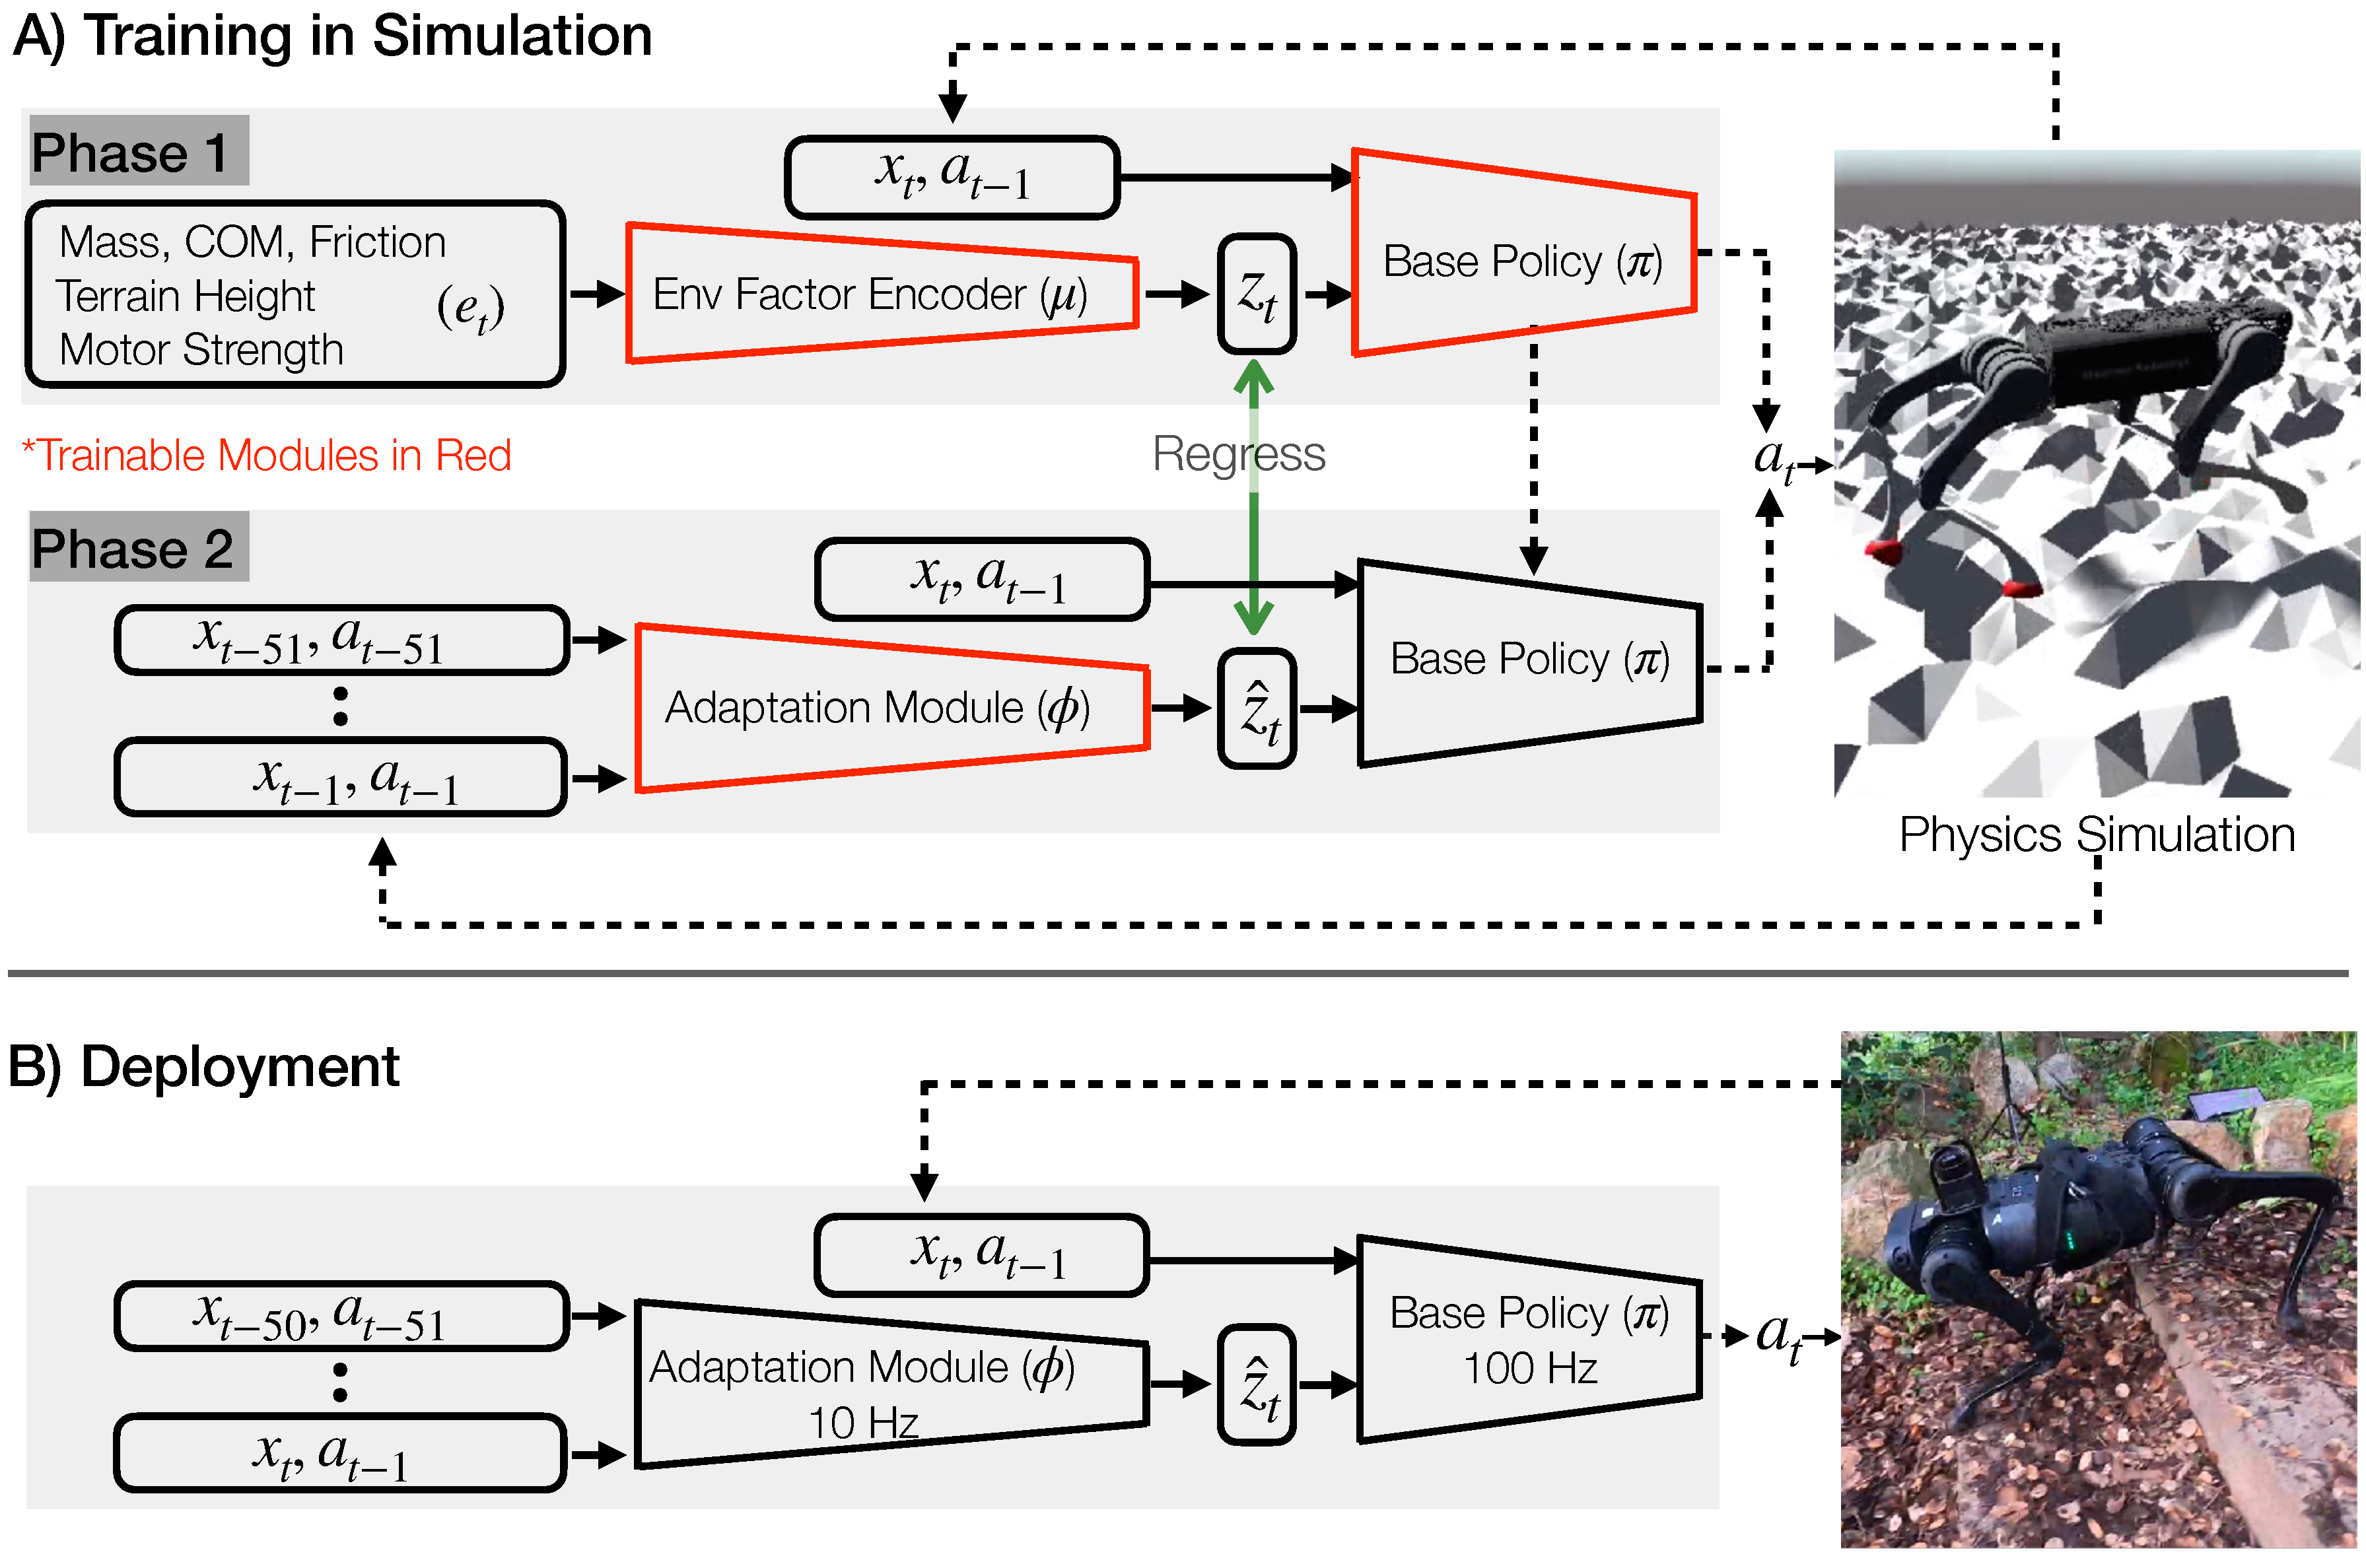
\includegraphics[height=56mm,keepaspectratio]{rma-method-1.pdf}

  \vspace{1.0mm}
  \raggedright
  {\scriptsize\color{muted}
  Figure~2 of the paper. Modules in red are trained. The upper half is the two phases in simulation; the lower half is deployment. $\phi$ runs at 10\,Hz and $\pi$ at 100\,Hz.}
\end{frame}

\begin{frame}{Phase 1 | Walk as if the context were known}
  \centering
  {\small $z_t = \mu(e_t)\in\mathbb{R}^{8}$\quad $\rightarrow$\quad $a_t = \pi(x_t, a_{t-1}, z_t)$}

  \vspace{0.7em}
  \begin{columns}[T,onlytextwidth]
    \begin{column}{0.32\textwidth}
      \infocard[blue]{$e_t$: 17-D}{Mass and center of mass, 3\\Motor strength, 12\\Friction 1, terrain height 1}
    \end{column}
    \hfill
    \begin{column}{0.32\textwidth}
      \infocard[orange]{$x_t$: 30-D}{Joint positions and velocities\\Torso roll and pitch\\Foot contacts}
    \end{column}
    \hfill
    \begin{column}{0.32\textwidth}
      \infocard[green]{$a_t$: 12-D}{Target joint angles\\Torque via PD\\$K_p=55$, $K_d=0.8$}
    \end{column}
  \end{columns}

  \vspace{0.85em}
  \metricbox[green]{15{,}000}{PPO iterations}\hspace{1.1em}%
  \metricbox[green]{24\,h}{one desktop}\hspace{1.1em}%
  \metricbox[green]{1.2\,B}{simulated steps}

  \takeaway{$z_t$ is a summary of how the gait should change, rather than a copy of friction or mass.}
  \source{Kumar et al., Sec.~3.1, Sec.~4.2}
\end{frame}

\begin{frame}{Phase 1 | No reference gait is provided}
  \begin{columns}[T,onlytextwidth]
    \begin{column}{0.34\textwidth}
      \infocard[orange]{No reference gait}{Forward speed is capped at 0.35\,m/s. No motion to imitate.}
    \end{column}
    \hfill
    \begin{column}{0.63\textwidth}
      \infocard[blue]{Penalized}{Lateral motion, yaw, work, and impact. Torque jerk, large actions, and joint speed. Tilt, vertical acceleration, and foot slip.}
    \end{column}
  \end{columns}

  \vspace{1.15em}
  \centering
  {\footnotesize\color{muted} Curriculum}\\[0.55em]
  \begin{tikzpicture}[node distance=6mm]
    \node[kwgreen, text width=32mm] (p) {penalties\\start small};
    \node[kwgreen, text width=34mm, right=of p] (q) {raise penalties\\and spread};
    \node[kwgreen, text width=34mm, right=of q] (r) {fractal terrain\\from the start};
    \draw[kwarr] (p) -- (q);
    \draw[kwarr] (q) -- (r);
  \end{tikzpicture}

  \takeaway{A reward built around work and impact, plus uneven terrain, produces a gait without reference trajectories.}
  \source{Kumar et al., Sec.~3.1}
\end{frame}

\begin{frame}{Phase 2 | Estimate $z_t$ from the last half-second}
  \centering
  {\small $\hat z_t = \phi(x_{t-50:t-1}, a_{t-50:t-1})$}
  \quad{\footnotesize\color{muted} 50 steps $=$ 0.5\,s \quad 1-D CNN \quad MSE}

  \vspace{0.85em}
  \begin{columns}[T,onlytextwidth]
    \begin{column}{0.48\textwidth}
      \infocard[blue]{Collect with the true $z_t$}{Only clean walking remains. $\phi$ never sees a disturbed gait.}
    \end{column}
    \hfill
    \begin{column}{0.48\textwidth}
      \infocard[orange]{RMA: collect with $\hat z_t$}{Failed steps enter the data. $\phi$ is updated against the true $z_t$ by MSE.}
    \end{column}
  \end{columns}

  \vspace{0.9em}
  \centering
  {\footnotesize\color{muted} 1{,}000 iterations \quad about 3\,h \quad 80\,M steps}

  \takeaway{The target is the $z_t$ the policy uses, so a complete identification of the physical parameters is unnecessary.}
  \source{Kumar et al., Sec.~3.2}
\end{frame}

\begin{frame}{Deployment | Slow estimation and fast control on separate clocks}
  \centering
  \begin{tikzpicture}[node distance=8mm]
    \node[kwgreen, text width=32mm] (phi) {Adaptation $\phi$\\10\,Hz\\0.5\,s history};
    \node[kwgreen, text width=32mm, right=of phi] (pi) {Policy $\pi$\\100\,Hz\\latest $\hat z_t$};
    \node[kwgreen, text width=26mm, right=of pi] (a) {Joint targets\\$a_t$};
    \draw[kwarr] (phi) -- (pi);
    \draw[kwarr] (pi) -- (a);
  \end{tikzpicture}

  \vspace{0.7em}
  \begin{columns}[T,onlytextwidth]
    \begin{column}{0.48\textwidth}
      \infocard[blue]{One network on the history}{The gait turns unnatural. Onboard it only reaches 10\,Hz, and the two rates must be aligned.}
    \end{column}
    \hfill
    \begin{column}{0.48\textwidth}
      \infocard[orange]{RMA's two clocks}{No shared clock. Deployed on the A1 (12\,kg, 12 actuators) with no calibration and no fine-tuning.}
    \end{column}
  \end{columns}

  \takeaway{Separating the slow context from the fast body is what makes the controller fit a low-cost robot.}
  \source{Kumar et al., Sec.~3.3}
\end{frame}

\begin{frame}{Experiments | Isolate the adaptation module}
  \centering
  {\footnotesize
  \begin{tabular}{lll}
    \toprule
    Method & What is passed at runtime & Extra real samples \\
    \midrule
    Robust & nothing (randomization only) & 0 \\
    SysID & a prediction of $e_t$ itself & 0 \\
    AWR & $\hat z_t$ optimized afterwards & 40k \\
    \textbf{RMA} & $\hat z_t$ from recent history & \textbf{0} \\
    \midrule
    Expert & the true $z_t$ (upper bound) & 0 \\
    \bottomrule
  \end{tabular}}

  \vspace{0.7em}
  \raggedright
  \begin{columns}[T,onlytextwidth]
    \begin{column}{0.48\textwidth}
      \infocard[green]{In simulation}{Reward and network stay fixed. What changes is whether $z_t$ is used, and how it is made.}
    \end{column}
    \hfill
    \begin{column}{0.48\textwidth}
      \infocard[orange]{On the robot}{The A1 force-based MPC, and RMA with adaptation off. Five trials indoors.}
    \end{column}
  \end{columns}

  \takeaway{Reward and network structure stay fixed. What changes is whether $z_t$ is used, and how it is produced.}
  \source{Kumar et al., Sec.~5}
\end{frame}

\begin{frame}{Simulation | Success close to the true extrinsics}
  \vspace{0.2em}
  \centering
  {\footnotesize
  \begin{tabular}{lcccc}
    \toprule
     & Success (\%) & TTF & Reward & Distance (m) \\
    \midrule
    Robust & 62.4 & 0.80 & 4.62 & 1.13 \\
    SysID & 56.5 & 0.74 & 4.82 & 1.17 \\
    AWR & 41.7 & 0.65 & 4.17 & 0.95 \\
    w/o adaptation & 52.1 & 0.75 & 4.72 & 1.15 \\
    \textbf{RMA} & \textbf{73.5} & \textbf{0.85} & \textbf{5.22} & \textbf{1.34} \\
    \midrule
    Expert (bound) & 76.2 & 0.86 & 5.23 & 1.35 \\
    \bottomrule
  \end{tabular}}

  \vspace{0.7em}
  \raggedright
  {\small
  During testing, environment parameters are redrawn with probability 0.01 at each step. AWR needs 40{,}000 samples to adapt. RMA needs none.}

  \takeaway{When the context keeps changing, post-hoc optimization and direct estimation of $e_t$ both fall behind an estimate of $z_t$.}
  \source{Kumar et al., Table~2, Sec.~5.3. Mean over 3 seeds and 1{,}000 episodes each.}
\end{frame}

\begin{frame}{Hardware | Steps, soft ground, and payload indoors}
  \centering
  {\footnotesize
  \begin{tabular}{cccc}
    \toprule
    80\% & 100\% & 12\,kg & 90\% \\
    \midrule
    step down 15\,cm & foam and mattress & payload cap (A1: 8\,kg) & oily sheet \\
    \bottomrule
  \end{tabular}}

  \vspace{1.05em}
  \begin{columns}[T,onlytextwidth]
    \begin{column}{0.48\textwidth}
      \infocard[orange]{Flat floor}{Without adaptation the policy already walks, and no calibration is used.}
    \end{column}
    \hfill
    \begin{column}{0.48\textwidth}
      \infocard[blue]{Adaptation removed}{Falls stay rare. Forward progress stops.}
    \end{column}
  \end{columns}

  \takeaway{One deployed policy retargets its gait for load, steps, and slip.}
  \source{Kumar et al., Fig.~3, Sec.~5.1}
\end{frame}

\begin{frame}{Hardware | Stairs and sand never appear in training}
  \centering
  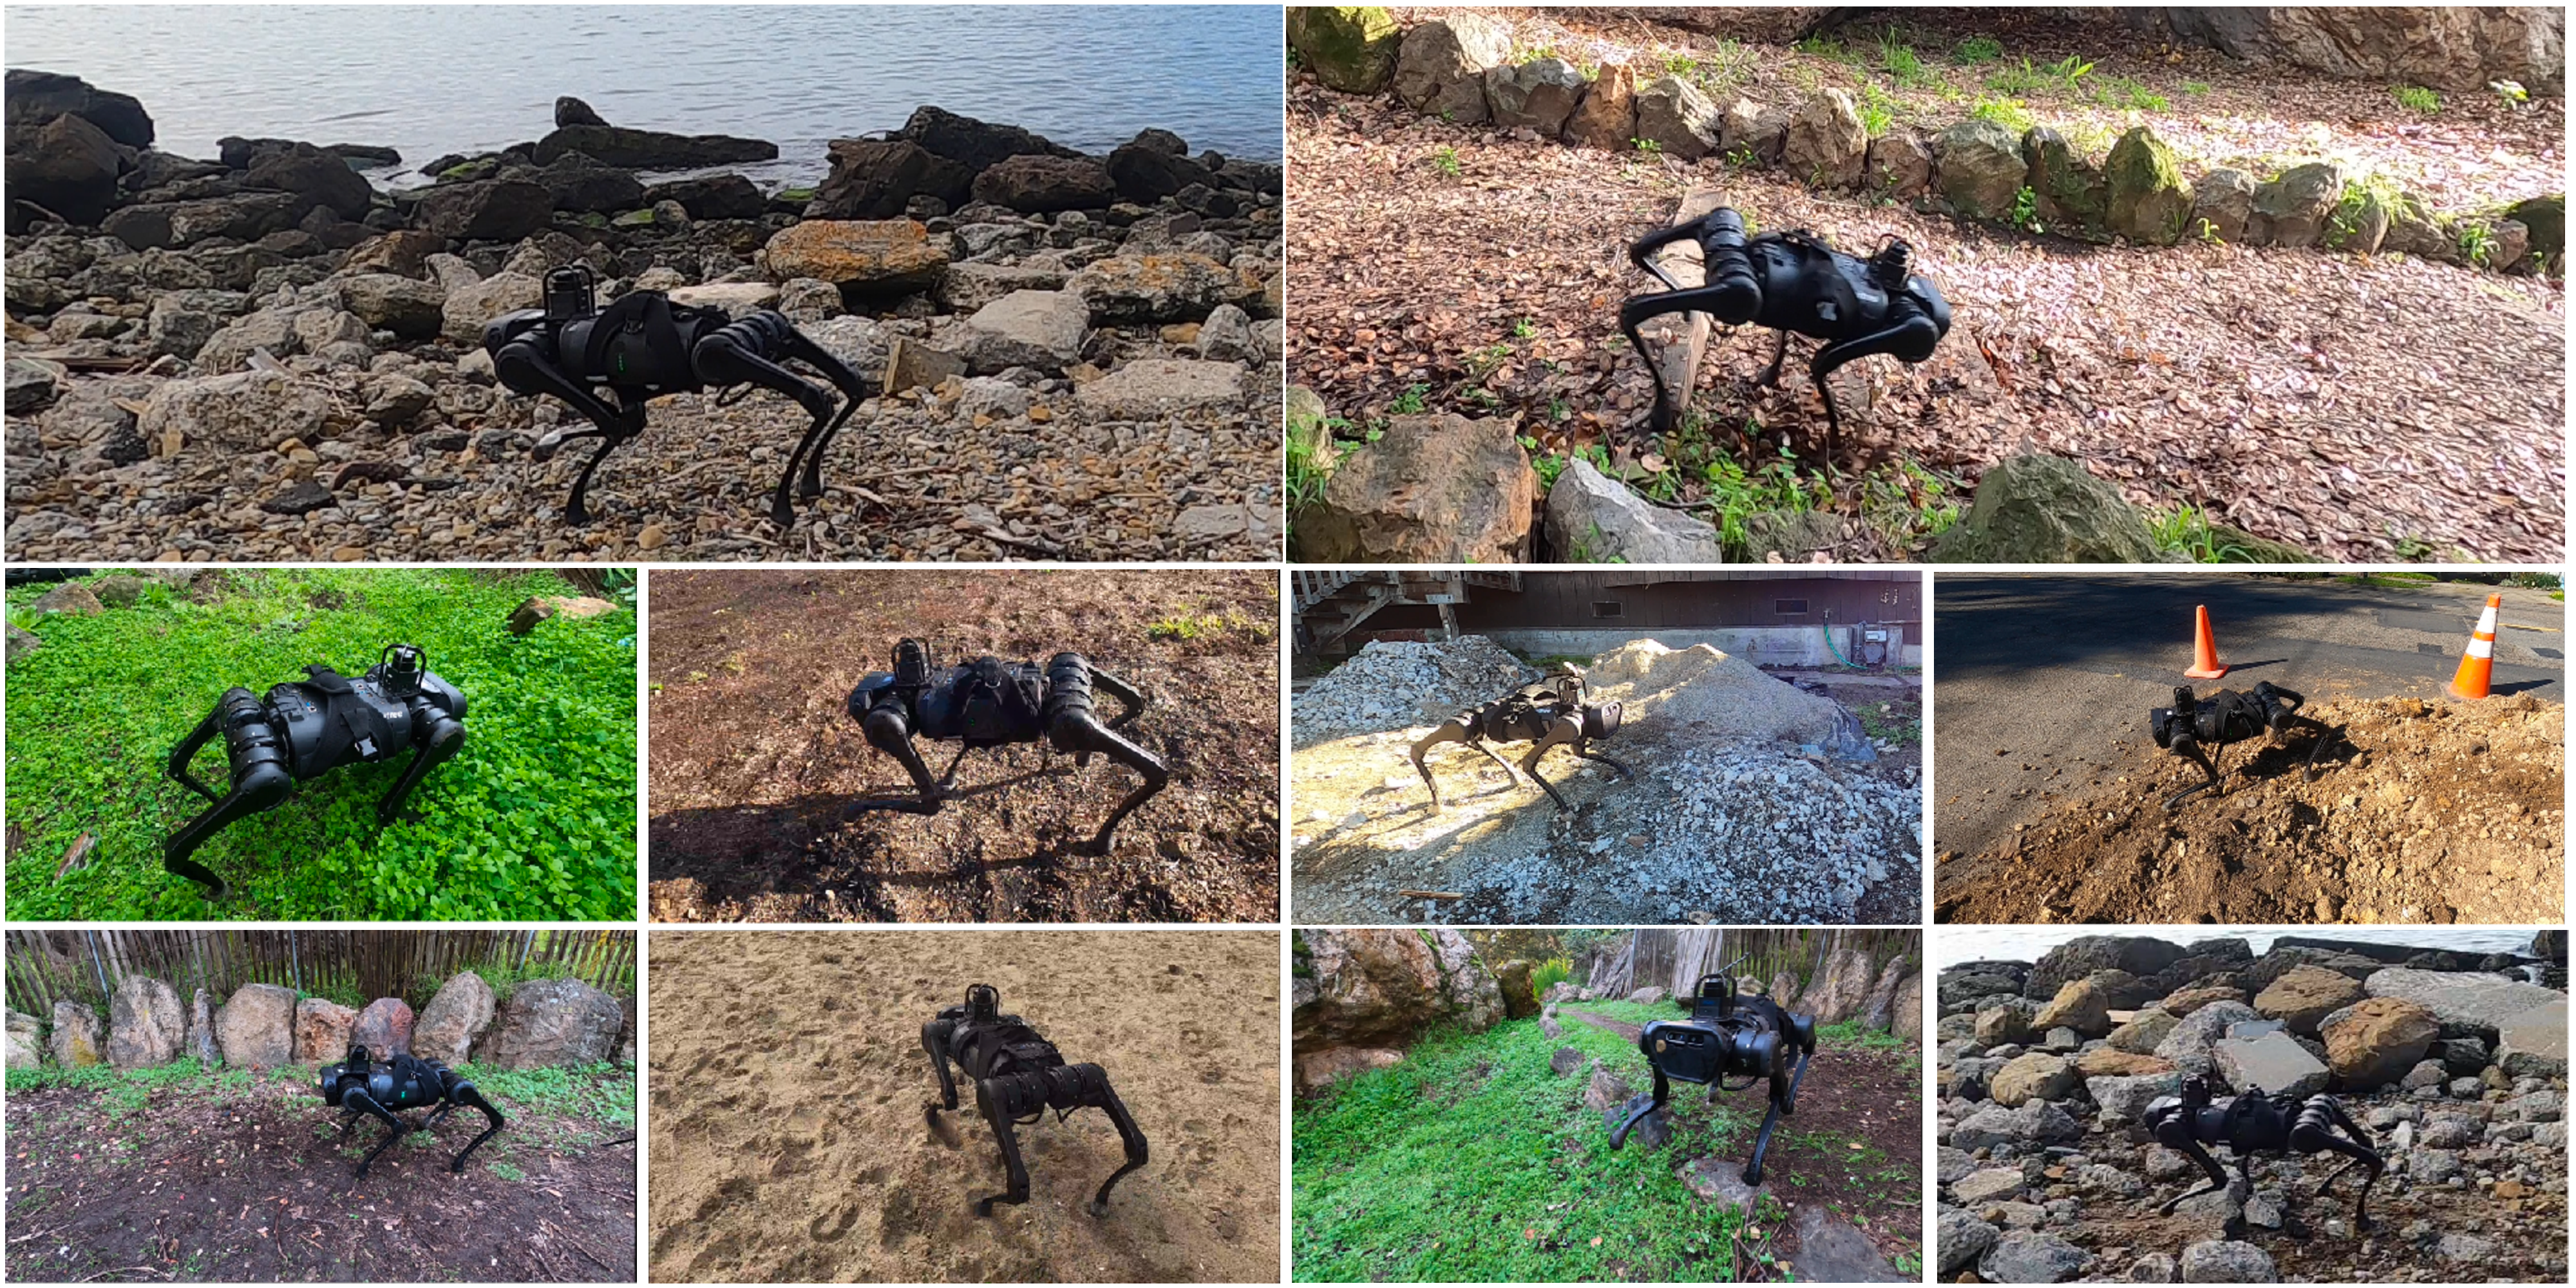
\includegraphics[width=0.72\textwidth,keepaspectratio]{outdoors-alt.pdf}

  \vspace{0.8mm}
  \raggedright
  {\small
  Sand, mud, dirt, tall grass, and bushes produced no failures in the reported trials. Downhill stairs on a hiking trail succeed in 70\% of trials, and a cement pile with pebbles in 80\%. Stairs are absent from training.}

  \source{Kumar et al., Fig.~1, Sec.~5.2. Videos: \url{https://ashish-kmr.github.io/rma-legged-robots/}}
\end{frame}

\begin{frame}{Analysis | Slip stays visible in $\hat z$}
  \begin{columns}[c,onlytextwidth]
    \begin{column}{0.40\textwidth}
      \begin{itemize}
        \item Near 2\,s the feet begin to slip, the gait breaks, and components of $\hat z$ move.
        \item After recovery, torque is slightly higher and the period is close to the original.
        \item $\hat z$ does not return to its old value. It keeps the fact that the surface is still slippery.
      \end{itemize}
    \end{column}
    \begin{column}{0.58\textwidth}
      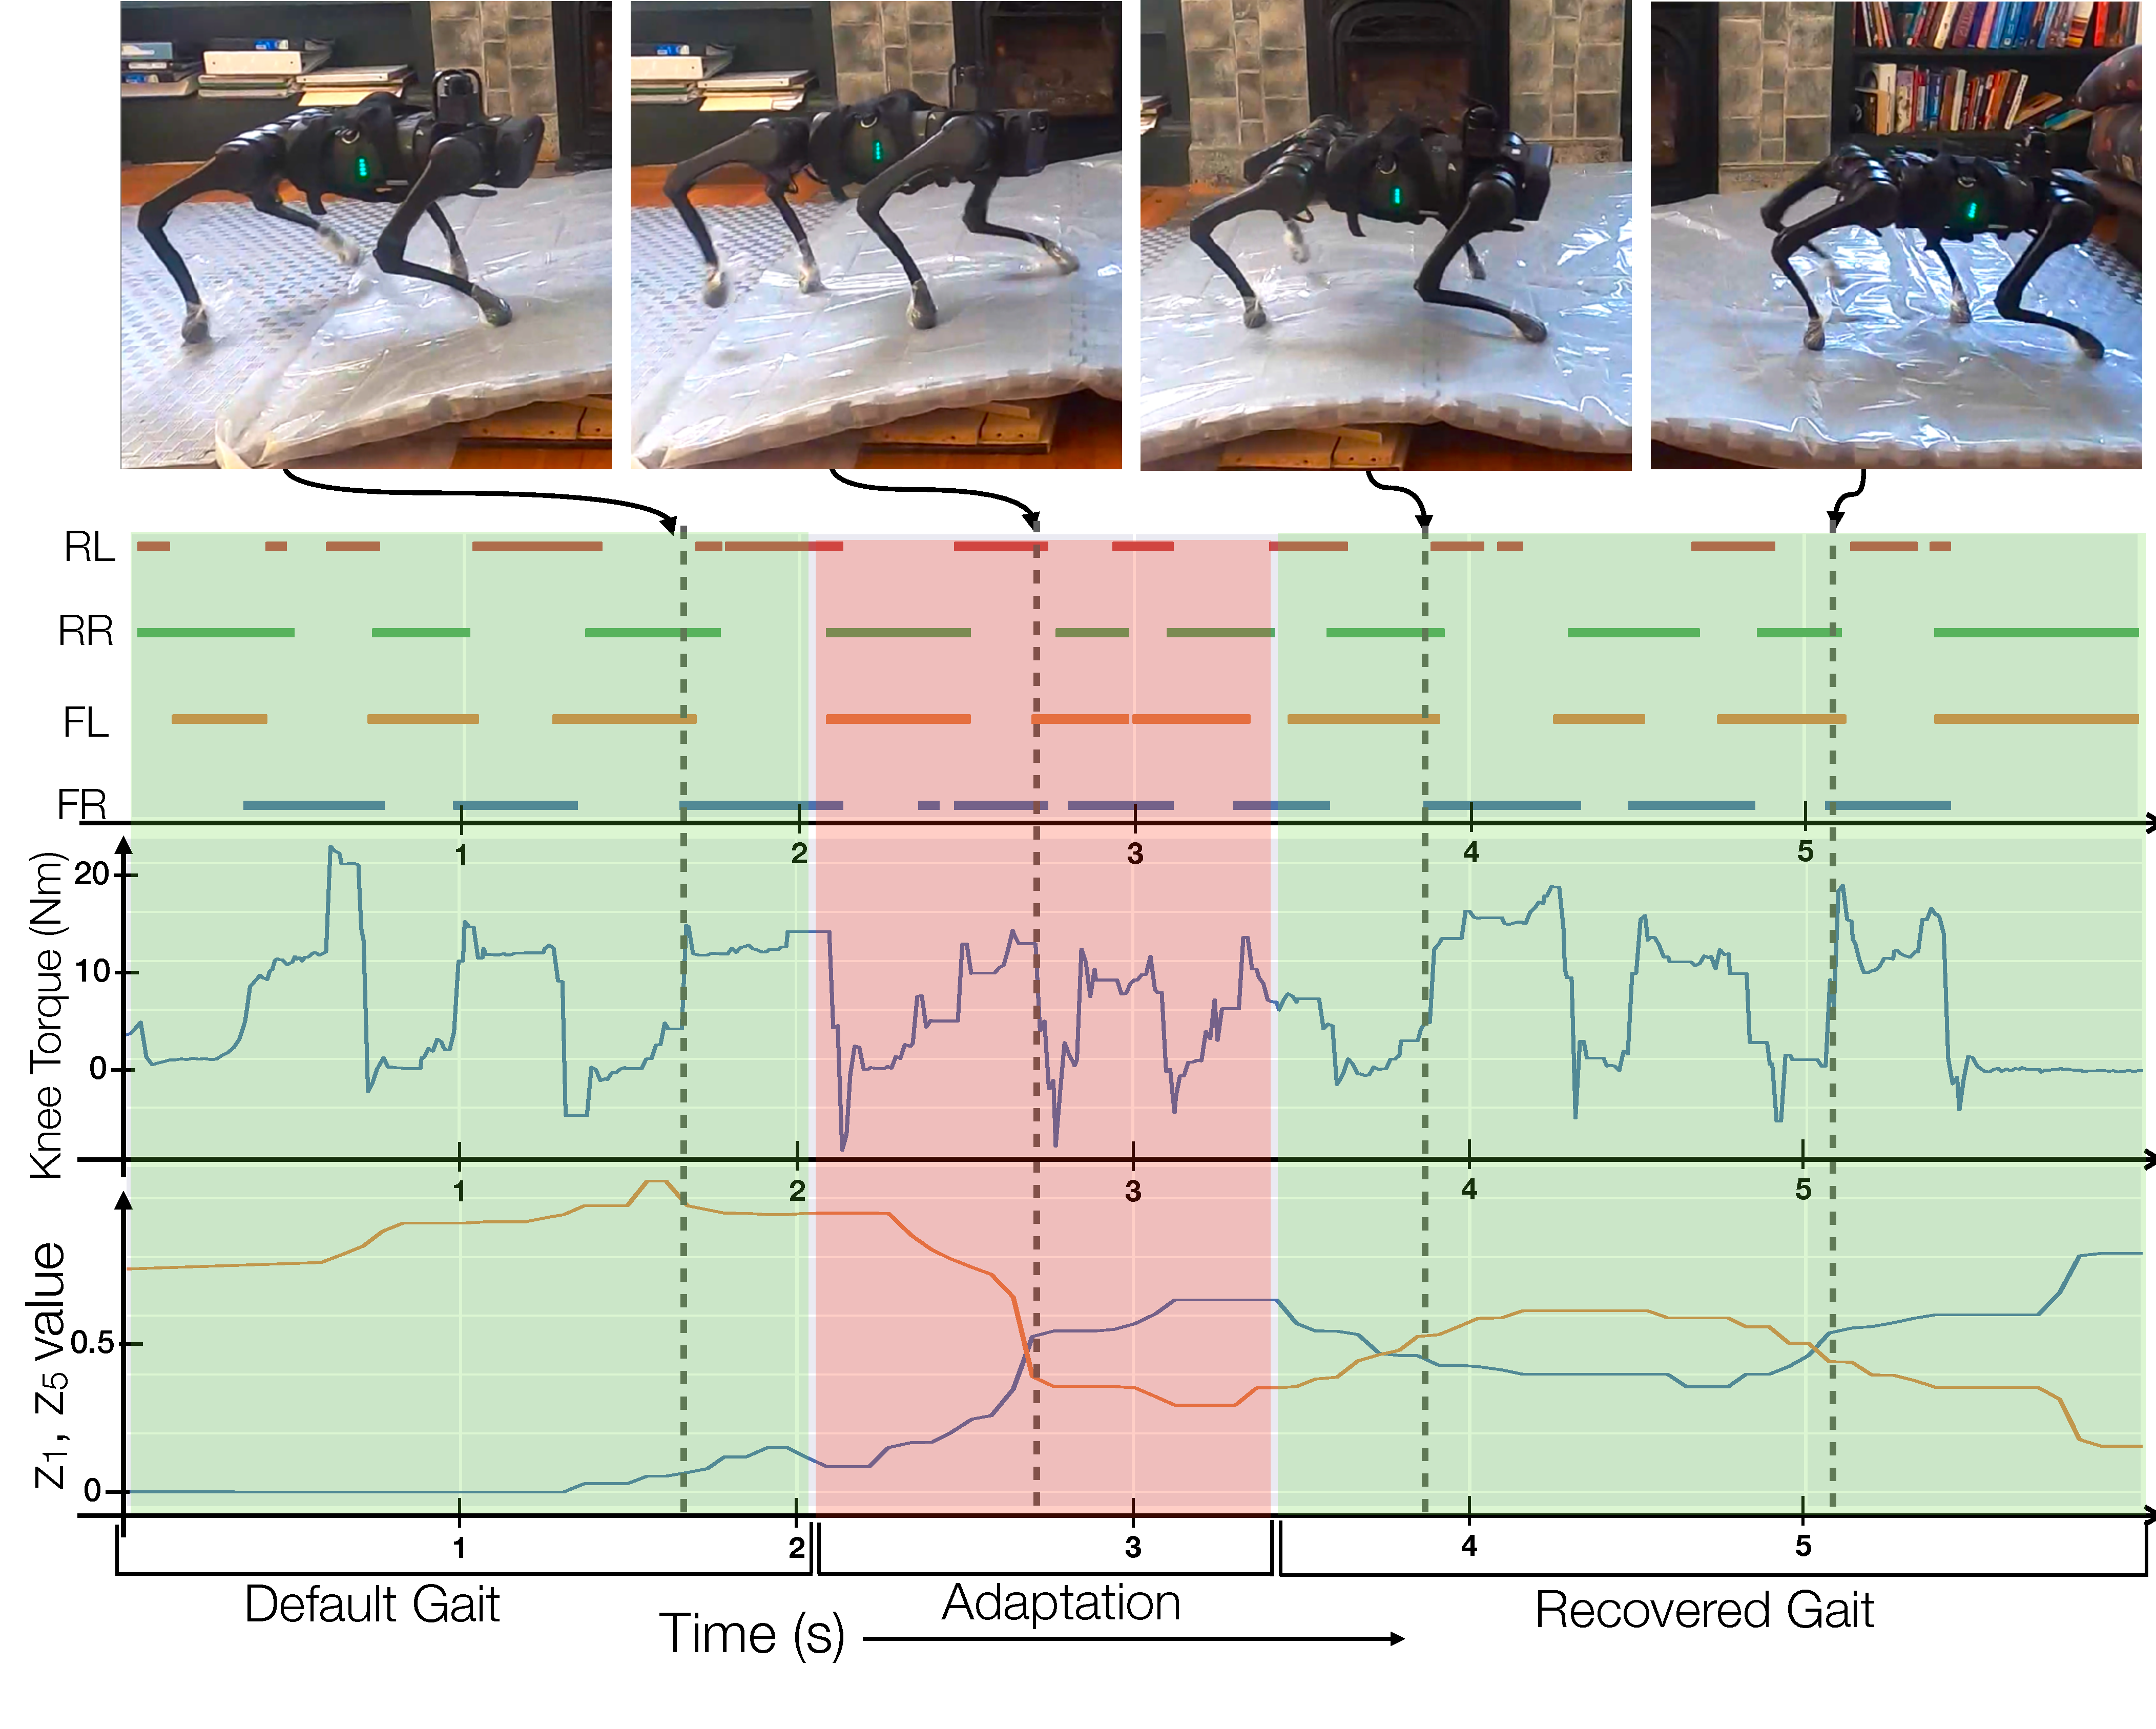
\includegraphics[height=46mm,keepaspectratio]{friction-analysis-fig.pdf}
    \end{column}
  \end{columns}
  \takeaway{The estimate is doing its job when it remains a cue for changing the gait.}
  \source{Kumar et al., Fig.~4, Sec.~5.4. Success on the oily sheet is 90\%.}
\end{frame}

\begin{frame}{Summary | Adaptation is not an optimization run at deployment}
  \begin{columns}[T,onlytextwidth]
    \begin{column}{0.32\textwidth}
      \infocard[orange]{What is learned}{The policy uses privileged $e_t$. At runtime, $z_t$ comes from 0.5\,s of history.}
    \end{column}
    \hfill
    \begin{column}{0.32\textwidth}
      \infocard[green]{Left unused}{Reference motions. Real-world fine-tuning. Simulator calibration.}
    \end{column}
    \hfill
    \begin{column}{0.32\textwidth}
      \infocard[blue]{What remains}{Proprioception only. Large falls and multi-leg snags still fail. The next sensor is vision.}
    \end{column}
  \end{columns}

  \vspace{0.9em}
  \centering
  \metricbox[orange]{73.5\%}{in simulation\\Expert is 76.2\%}\hspace{1.4em}%
  \metricbox[green]{sand, mud, grass}{steps, and a body-weight load}

  \takeaway{The useful split is a fast loop for the body and a slow loop for the context.}
  \source{Kumar et al., Sec.~6}
\end{frame}

\begin{frame}{References}
  {\footnotesize
  \begin{enumerate}
    \item Kumar, Fu, Pathak, Malik.
      \textbf{RMA: Rapid Motor Adaptation for Legged Robots.}
      RSS 2021.\\
      \url{https://arxiv.org/abs/2107.04034}
      \quad
      \url{https://ashish-kmr.github.io/rma-legged-robots/}
    \item Peng et al. Learning Agile Robotic Locomotion Skills by Imitating Animals. RSS 2020.
    \item Lee et al. Learning Quadrupedal Locomotion over Challenging Terrain. Science Robotics, 2020.
    \item Hwangbo et al. Learning Agile and Dynamic Motor Skills for Legged Robots. Science Robotics, 2019.
    \item Yu et al. Preparing for the Unknown: Learning a Universal Policy with Online System Identification. RSS 2017.
    \item Tobin et al. Domain Randomization for Transferring Deep Neural Networks from Simulation to the Real World. IROS 2017.
  \end{enumerate}}
\end{frame}

\end{document}
